The elastically-scattered electrons provided the clearest point in extracting the energy resolution of the ECal at the beam energy. Using WAB particles, electrons and photons, the energy resolution of the ECal was fully characterized in terms of energy and position relative to the edges.\\
\indent To study the energy resolution in the fiducial region of the ECal, all electrons were matched to tracks, and the track position extrapolation to the face of the ECal was used to determine the electron's vertical distance relative to the beam gap edge. For WAB electrons, the photon cluster was required to be at least 10~mm from the ECal edges to avoid edge effects. By selecting WAB events where the energy difference between the two particles is less than 100~MeV, the resolution of the energy sum peak was fitted to extract the resolution. The resolution was extracted according to Equation~\eqref{eq:eResExtract}.

\begin{equation}
	\label{eq:eResExtract}
	\sigma_{E_{\gamma}+E_{e-}}^2 = \sigma_{e-}^2(E_{e-})+\sigma_{\gamma}^2(E_{\gamma})
\end{equation}

When both particles are in the fiducial region and are roughly equal in energy, then the energy resolution of the sum could be divided by $\sqrt{2}$ assuming that the energy resolution of both particles is the same. This same procedure was used to study the resolution when the particle energies were more asymmetric in energy in order to obtain the single particle energy resolution at various energies. \\
\indent The experimentally-obtained fiducial energy resolution agrees well with Monte Carlo but generally yields a larger energy resolution across all energies (on the order of about 15$\%$). The energy resolution obtained in data is shown in Figure~\ref{Figure:eResData}.

\begin{figure}[H]
  \centering
      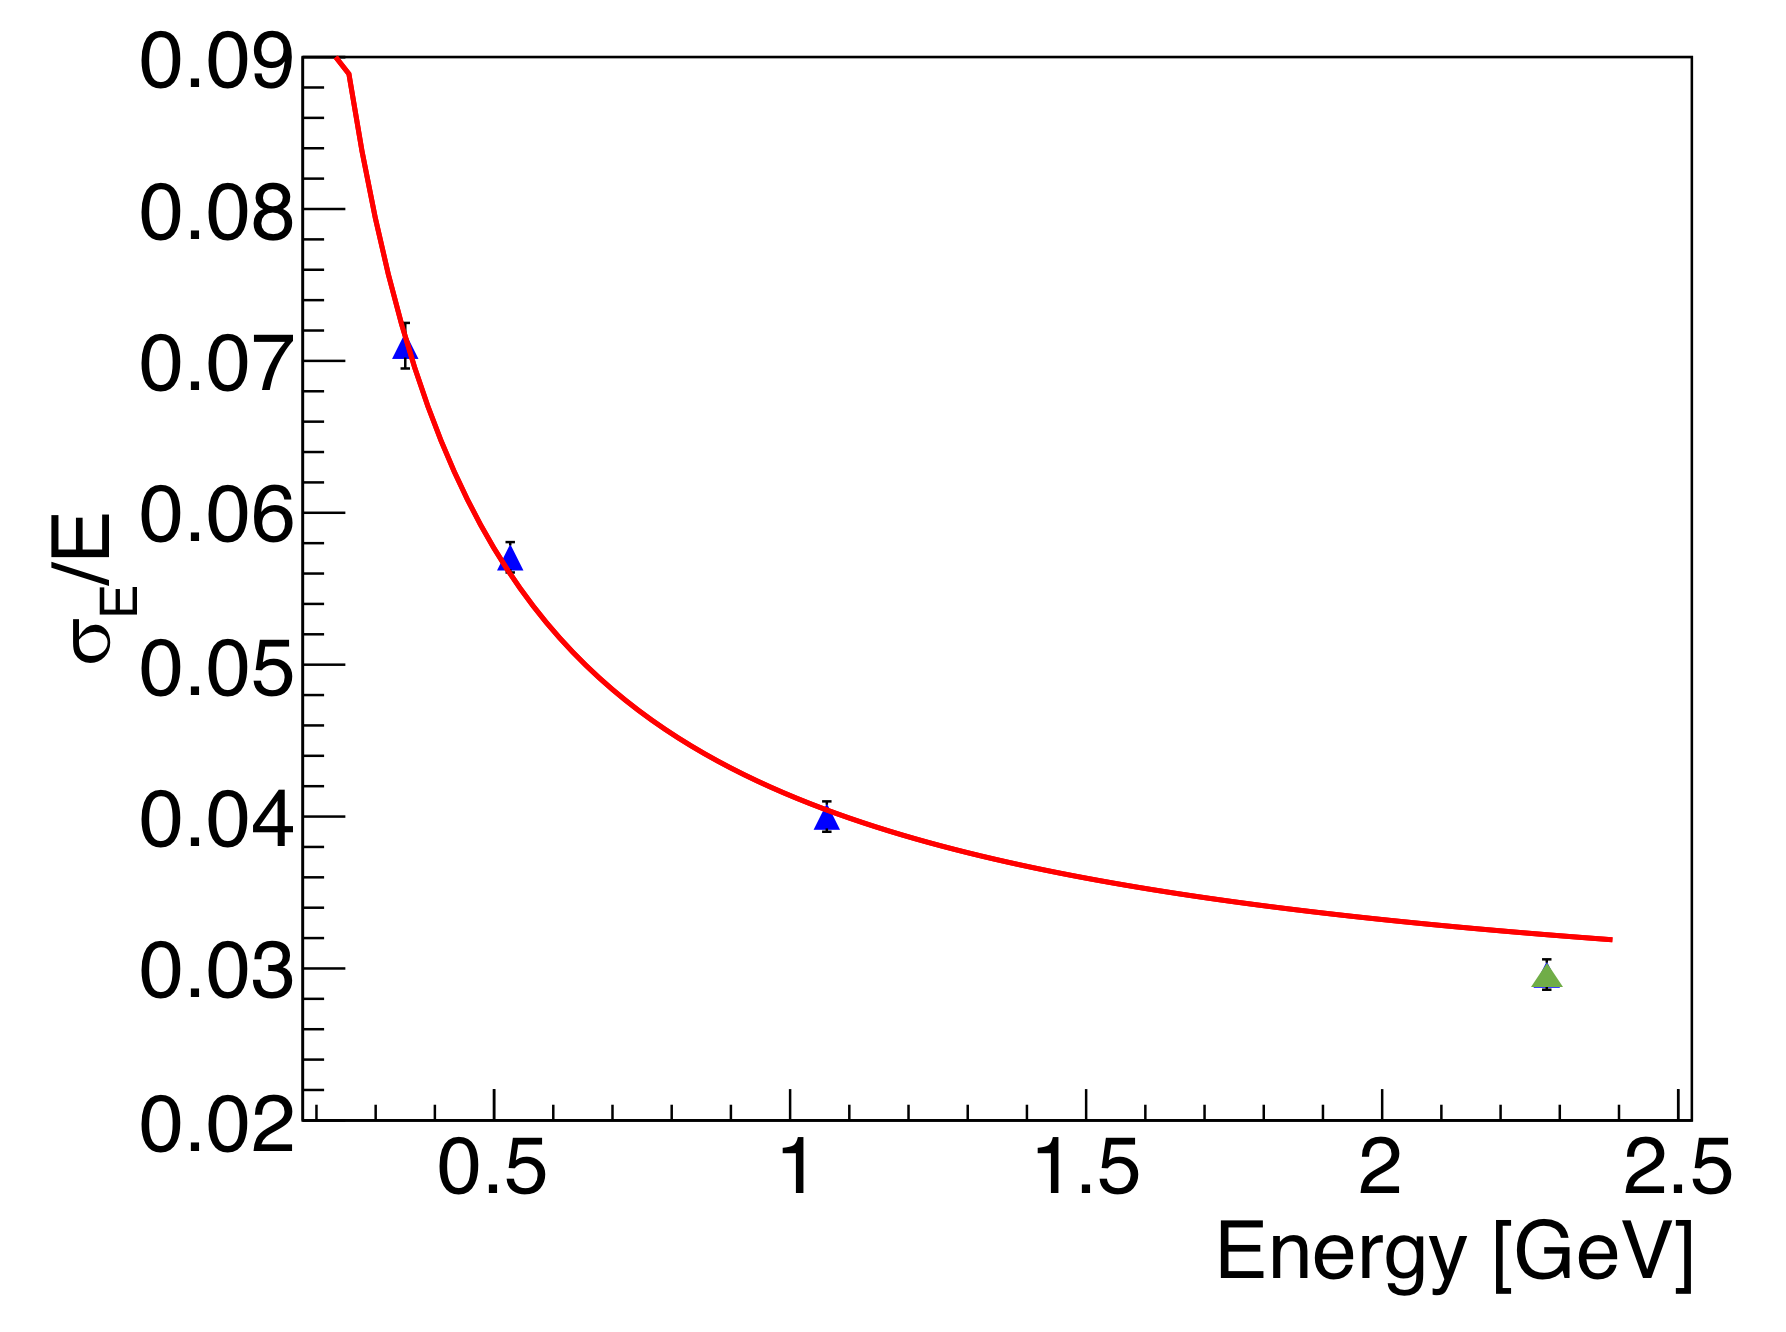
\includegraphics[width=0.6\textwidth]{pics/performance/eResData.png}
  \caption[Energy resolution of the ECal found in data]{The blue points are derived from the Engineering Run for the energy resolution of a single particle. The green point at approximately 2.3~GeV was determined from the elastic calibration of the Physics Run data. The fitted energy resolution was determined from the Engineering Run data only, but it shown here extrapolated to higher energies.}
  \label{Figure:eResData}
\end{figure}

The fit to the energy resolution in data is shown in Equation~\eqref{eq:eResData} and uses the blue points from the Engineering Run data in Figure~\ref{Figure:eResData}.

\begin{equation}
	\label{eq:eResData}
	\dfrac{\sigma_E}{E}(\%) = \dfrac{1.62}{E}\oplus\dfrac{2.87}{\sqrt{E}}\oplus2.5
\end{equation}

The first term in Equation~\eqref{eq:eResData} is attributed to the noise from the pre-amplifiers and is roughly consistent to that found in Monte Carlo. The second term is related to the statistical fluctuations of the shower containment and the APD gain. This term is larger than the term found in Monte Carlo but is still consistent. The third term contains both the energy leakage out the back of the ECal as well as the crystal-to-crystal inter-calibration error. This term is significantly higher than anticipated from Monte Carlo, but is comparable to that found for the IC. It's possible that this term is affected by the inability to calibrate several crystals along the outer edges of the calorimeter with elastics. \\
\indent The energy resolution from the Physics Run (shown in green on Figure~\ref{Figure:eResData}) is slightly better than that predicted by the fit from the Engineering Run It is likely that the energy resolution of the ECal improved overall because the signal going into the FADC modules was no longer split with TDC modules. \\
\indent The WAB events were additionally a useful tool for studying the energy resolution in the ECal as a function of position relative to the edge. By selection a photon cluster in the fiducial region of the ECal, the energy resolution of the electron (position given by the track projection at the ECal) could be measured at various energies and characterized. For each mm in the vertical position relative to the edge at the beam gap, it was found that the second parameter of the energy resolution described by Equation~\eqref{eq:eResData} (of the form $b/\sqrt{E}$) was strongly correlated with the position. By fixing the other two terms to the values in the fiducial region, the value of the $b$ parameter was studied as a function of position. ~\cite{CalibNote} The final characterization of this value relative to the beam gap edge is shown in Figure~\ref{eq:finalRes}.~\cite{Balossino}

\begin{figure}[H]
  \centering
      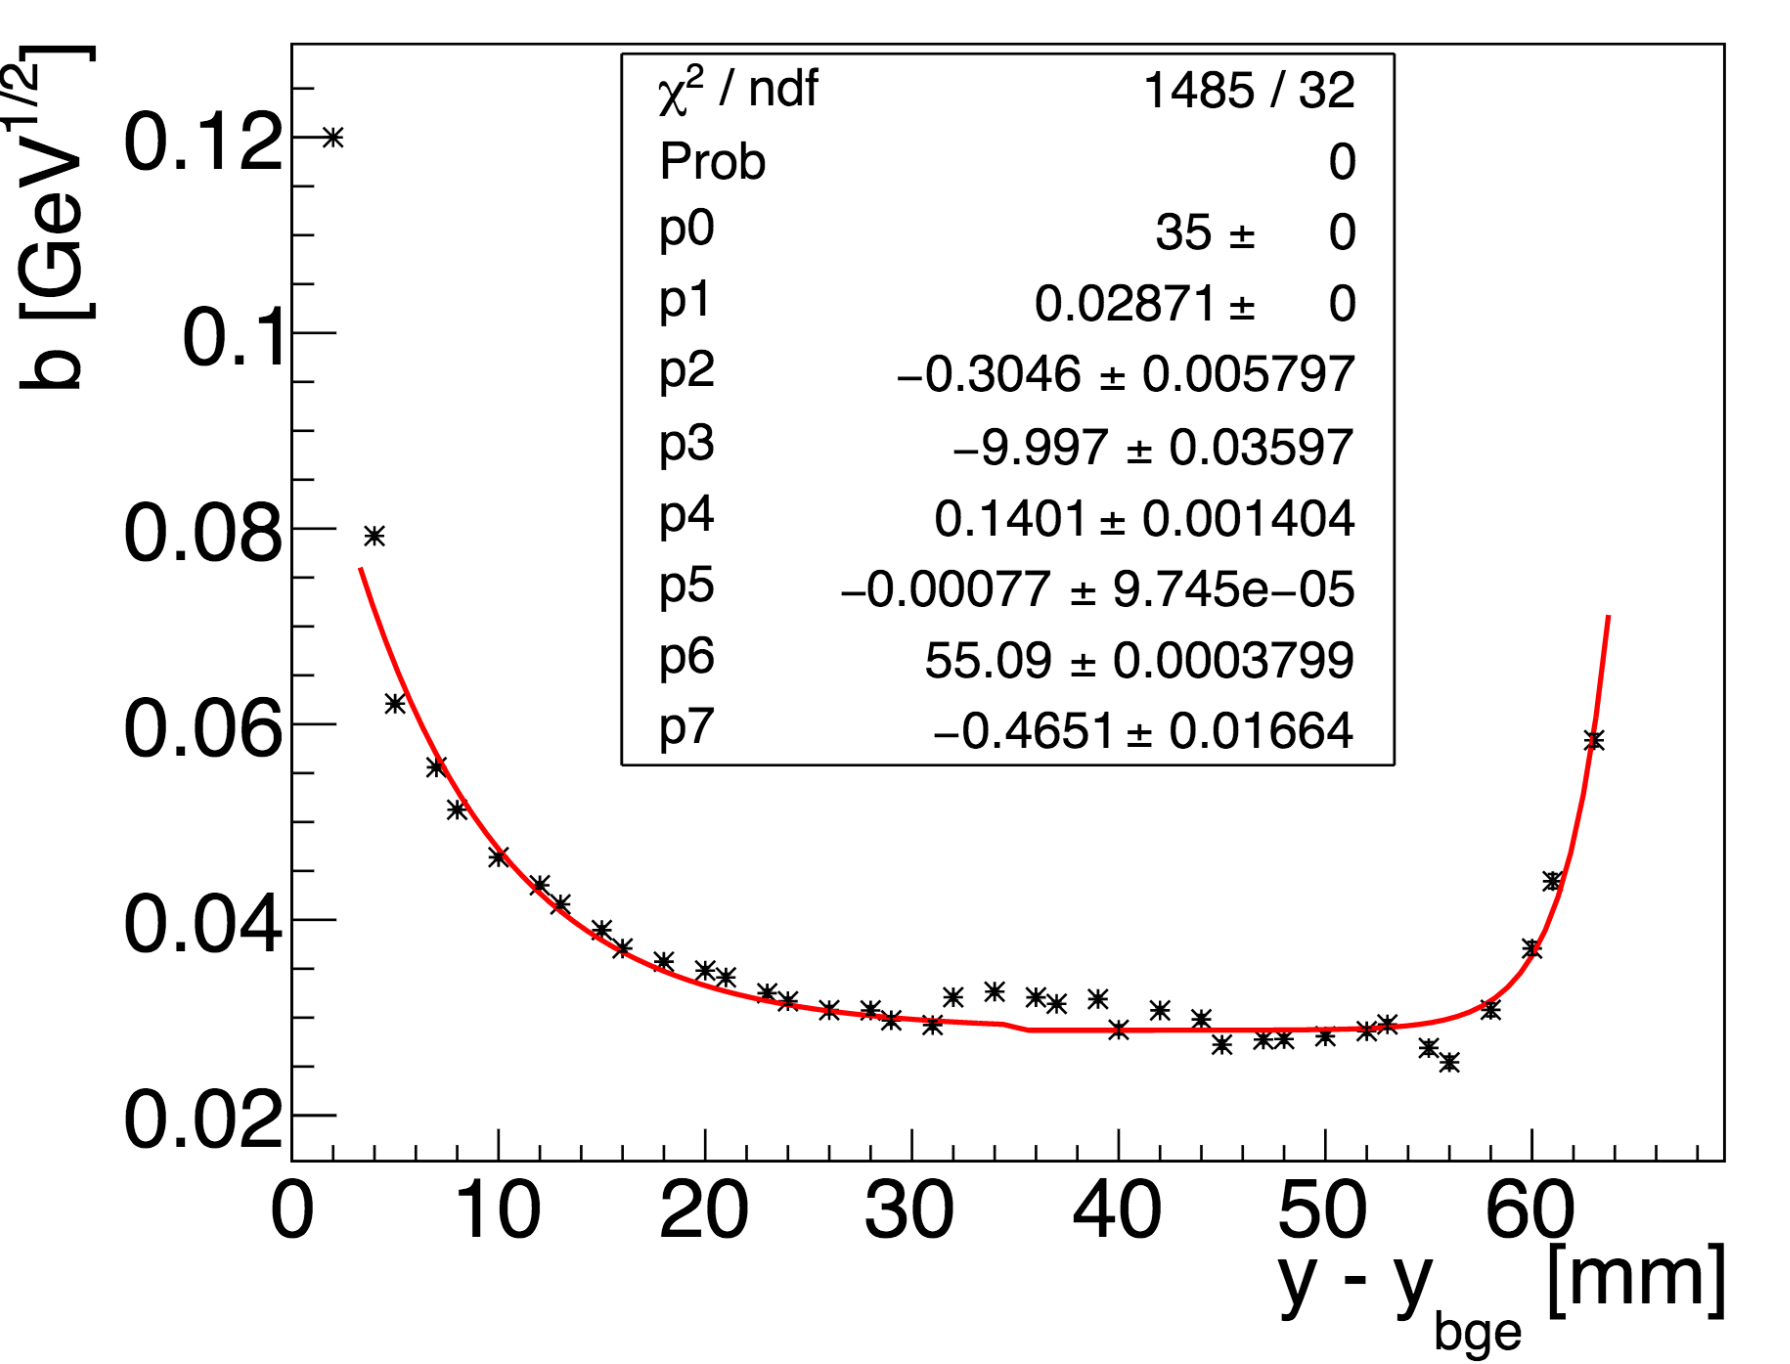
\includegraphics[width=0.5\textwidth]{pics/performance/eResEdgeEffect.png}
  \caption[Characterization of the energy resolution edge effects ]{The stochastic parameter $b$ (corresponding to the $1/\sqrt{E}$ term) of the energy resolution description is shown as a function of the vertical position relative to the ECal beam gap edge. The fit function is shown in Equation~\eqref{eq:finalRes}.}
  \label{Figure:stochasticEdge}
\end{figure}

The function that describes how Equation~\eqref{Figure:eResData} is modified to account for the position relative to the inner beam gap edge is shown in Equation~\eqref{eq:finalRes}.

\begin{equation}
\begin{split}
\label{eq:finalRes}
\dfrac{\sigma_E}{E}(\%)=\dfrac{1.62}{E}\oplus \dfrac{b(y-y_{bge})}{\sqrt{E}} \oplus 2.5 \\
B(y<p_0) = p_1-p_2 e^{-(y-p_3)p_4}\\
B(y>p_0) = p_1-p_5 e^{-(y-p_6)p_7}
\end{split}
\end{equation}

The energy resolution parameterizations are reliable down to approximately half a crystal width away from the edge of the crystal, but the energy is significantly deteriorating at about 10~mm from the edge of the crystal. ~\cite{CalibNote}
